\section{Introduction}

\subsection{Path planning}

\begin{frame}{Path planning}{Introduction}
	\begin{figure}
		\centering
		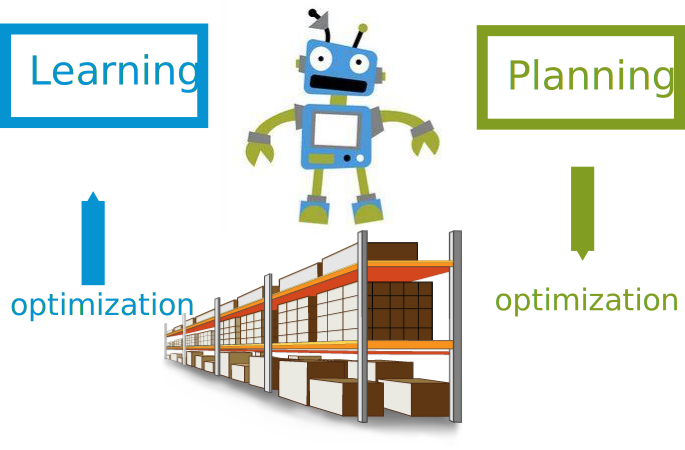
\includegraphics[width=.7\linewidth]{figure/robot_interaction}
		%\caption{}
		\label{fig:robot}
	\end{figure}
 \end{frame}

\begin{frame}{Path planning}{Introduction}
\begin{itemize}
\item Efficiency vs Optimality
\item Environment dynamics
\item Prior information modeling
\item Multiple agents
\item Human influence
\end{itemize}
\end{frame}

\subsection{Multi-objective optimization}

\begin{frame}{The need of multi-objective}{Introduction}
\begin{itemize}
\item Inherent {\em complexity} in tasks
\item From {\em cooperation} to {\em collaboration} (Robot independence)
\item {\em Communication} gap between the task supervisor and the task executor
\end{itemize}
\end{frame}

\begin{frame}{The need of multi-objective}{Introduction}
	\begin{figure}
		\centering
		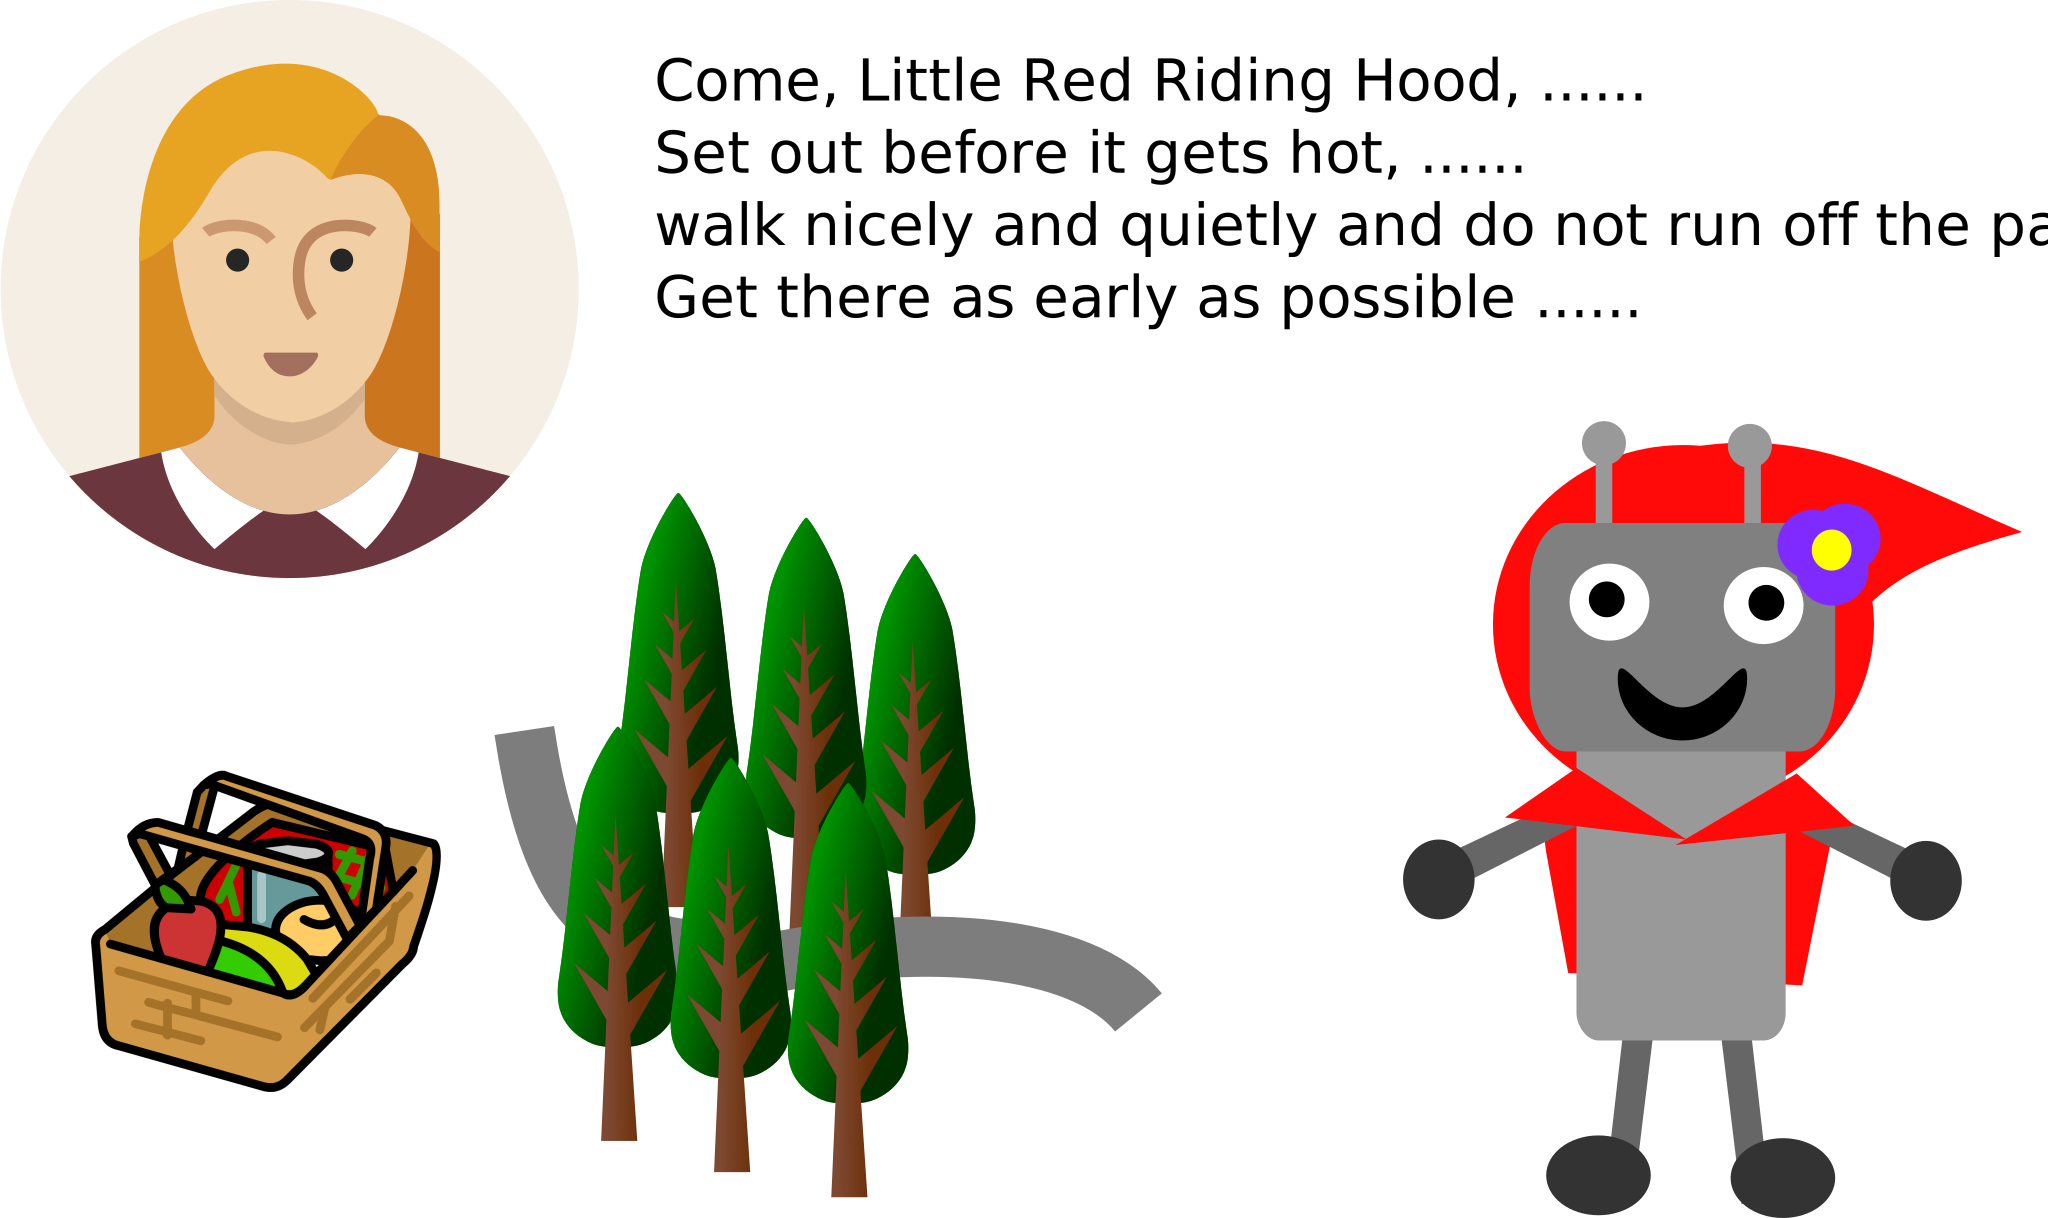
\includegraphics[width=\linewidth]{figure/task_assign}
		%\caption{}
		\label{fig:task_assign}
	\end{figure}
\end{frame}

\begin{frame}{The need of multi-objective}{Introduction}
Objectives
\begin{itemize}
\item \textbf{walk nicely}
\item \textbf{walk quietly}
\item \textbf{as early as possible}
\end{itemize}
Constraints
\begin{itemize}
\item  \textbf{set out before it gets hot}
\item \textbf{do not run off the path}
\end{itemize}
\end{frame}

\begin{frame}{The difficulty in multi-objective}{Introduction}
The problems in modeling human intent
\begin{itemize}
\item incomparability in objectives
\item conflict in objectives
\item hardness in weighing the objectives
\item vagueness in importance selection
\end{itemize}
\begin{figure}
	\centering
	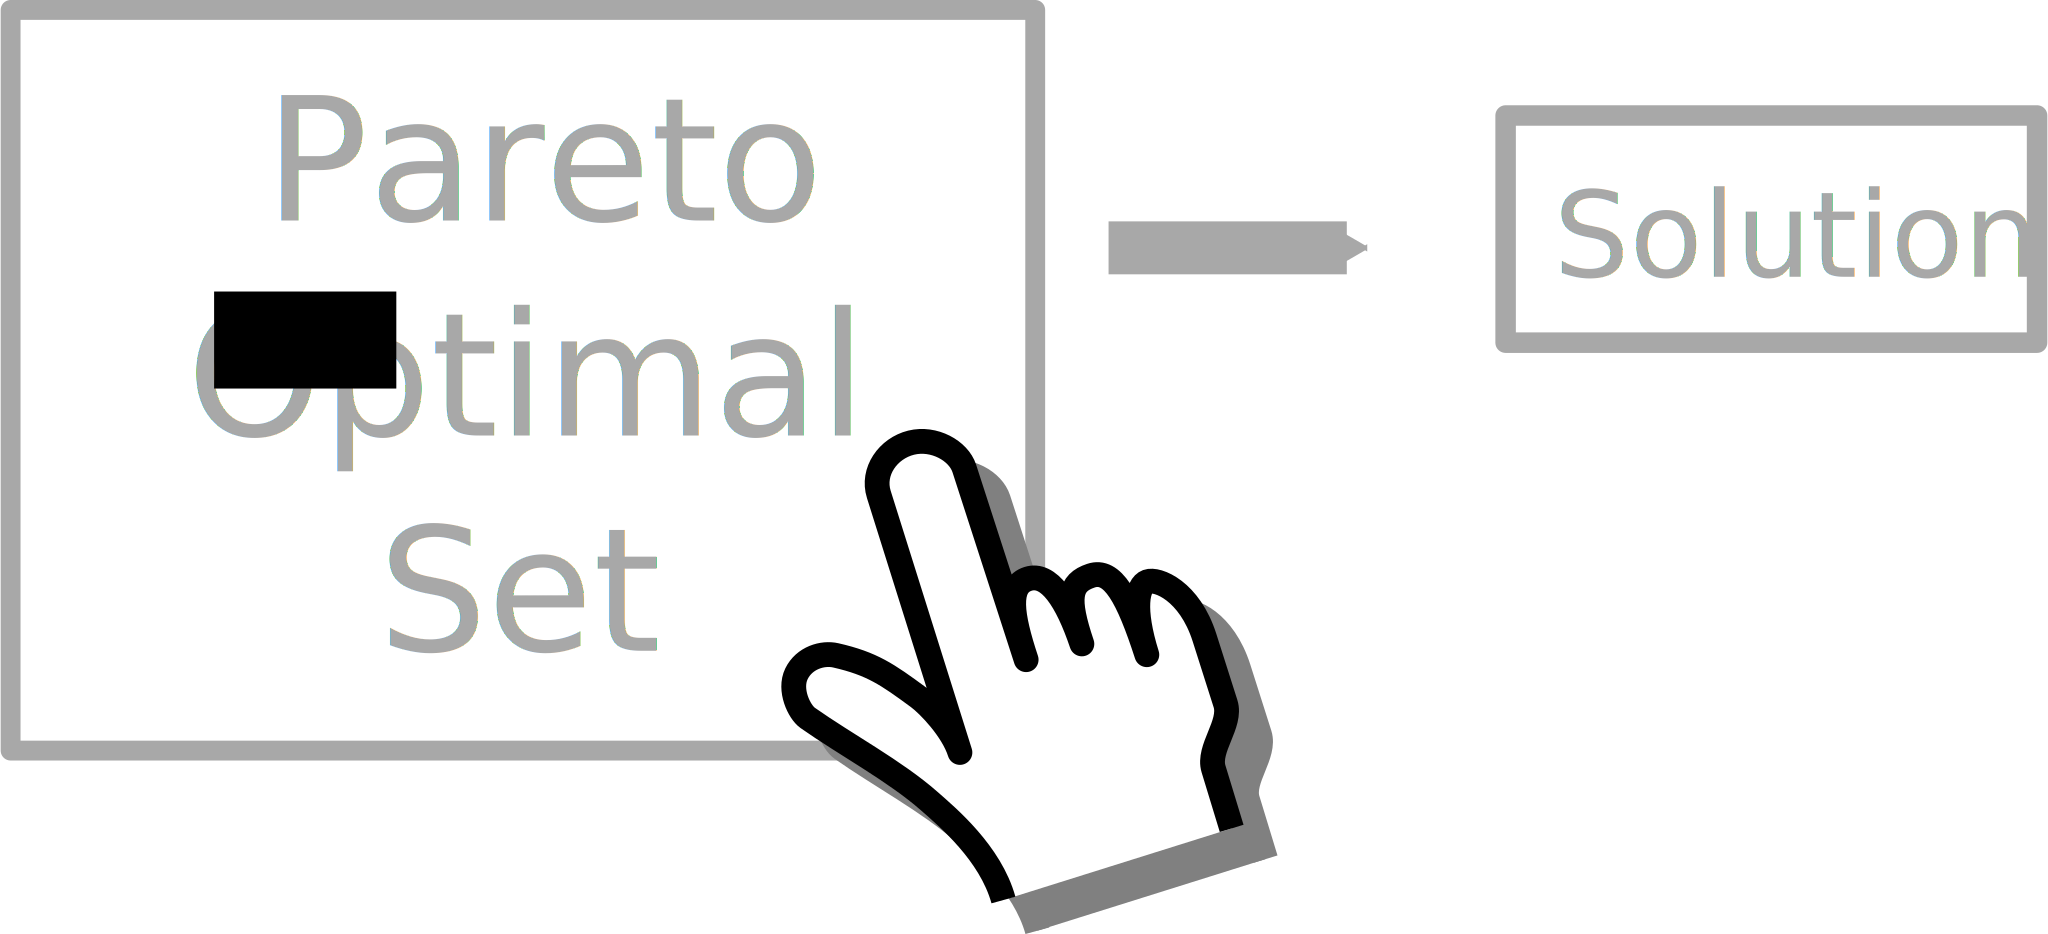
\includegraphics[width=0.6\linewidth]{figure/human_interactive_moo}
	%\caption{}
	\label{fig:human_interactive_moo}
\end{figure}
\end{frame}

\begin{frame}{Pareto Optimal}{Introduction}
%What is Pareto optimal
\begin{columns}
\column{0.5\textwidth}
	\begin{figure}
		\centering
		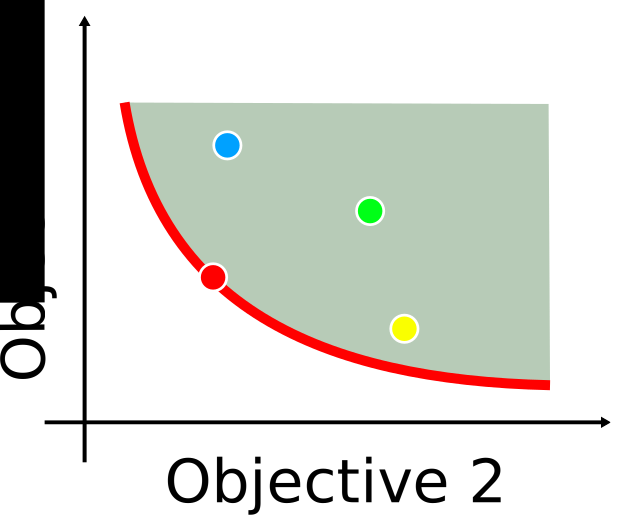
\includegraphics[width=\linewidth]{figure/pareto_optimal}
		%\caption{}
		\label{fig:pareot_optimal}
	\end{figure}
\column{0.5\textwidth}
\begin{minipage}{\textwidth}
\begin{itemize}
\item $ x_{a} \prec x_{b} $ (dominate)
\begin{eqnarray*}
\forall k, & f_{k} (x_{a}) \leq f_{k} (x_{b}) \\
\exists k, & f_{k} (x_{a}) < f_{k} (x_{b})
\end{eqnarray*}
\item non-dominance
\begin{eqnarray*}
\nexists x \in \mathbb{X}, x \prec x^{*}
\end{eqnarray*}
\end{itemize}
\end{minipage}
\end{columns}
\end{frame}

\begin{frame}{Hardness in finding Pareto optimal set}{Introduction}
Methods
\begin{itemize}
\item \emph{sorting based approach} : NSGA-II
\item \emph{decomposition based approach} : MOEA-D
\item \emph{approximation based approach} : PAES
\item \emph{sampling based approach} : ALP
\end{itemize}
\end{frame}

\begin{frame}{Hardness in finding Pareto optimal points}{Introduction}
\begin{columns}
\column{0.5\textwidth}
For the point representation
\begin{itemize}
\item constraints
\item discontinuity
\item nonconvex
\end{itemize}
\column{0.5\textwidth}
	\begin{figure}
		\centering
		\includegraphics[width=.6\linewidth]{figure/point_solution_space.png}
		%\caption{}
		\label{fig:point_solution_space}
	\end{figure}
	\begin{figure}
		\centering
		\includegraphics[width=.6\linewidth]{figure/point_fitness_space.png}
		%\caption{}
		\label{fig:point_fitness_space}
	\end{figure}
\end{columns}
\end{frame}

\begin{frame}{Hardness in finding Pareto optimal paths}{Introduction}
\begin{columns}
\column{0.5\textwidth}
For the path representation
\begin{itemize}
\item constraints
\item discontinuity
\item nonconvex
\item high dimension
\end{itemize}
\column{0.5\textwidth}
	\begin{figure}
		\centering
		%\nonumber
		\includegraphics[width=.6\linewidth]{figure/sim1-2obj/MORRTstar00-ALL.png}
		%\caption{Solutions pace}
		\label{fig:path_solution_space}
	\end{figure}
	\begin{figure}
		\centering
		\includegraphics[width=.6\linewidth]{figure/sim1-2obj/PF01-MORRT.png}
		%\caption{}
		\label{fig:path_fitness_space}
	\end{figure}
\end{columns}
\end{frame}